    
% !TEX TS-program = xelatex
% !TEX encoding = UTF-8 Unicode
% !Mode:: "TeX:UTF-8"

\documentclass{resume}
\usepackage{graphicx}
\usepackage{tabu}
\usepackage{tabularx}
\usepackage{multirow}
\usepackage{progressbar}
\usepackage{zh_CN-Adobefonts_external} % Simplified Chinese Support using external fonts (./fonts/zh_CN-Adobe/)
\usepackage{tikz}
% \usepackage{NotoSansSC_external}
% \usepackage{NotoSerifCJKsc_external}
% \usepackage{zh_CN-Adobefonts_internal} % Simplified Chinese Support using system fonts
\usepackage{linespacing_fix} % disable extra space before next section
\usepackage{cite}

\newcommand{\hlink}[1]{\href{#1}{#1}}

\begin{document}
\pagenumbering{gobble} % suppress displaying page number

\medskip\noindent
\begin{minipage}{0.7\textwidth}
  \Large{
    \begin{tabu}  { l }
      \scshape{曹\quad 东} \\
      \email{caodong0521@163.com} \\
      \phone{(+86) 188-1017-5210} \\
    \end{tabu}
  }
\end{minipage}
\begin{minipage}{0.3\textwidth}
  \raggedleft
  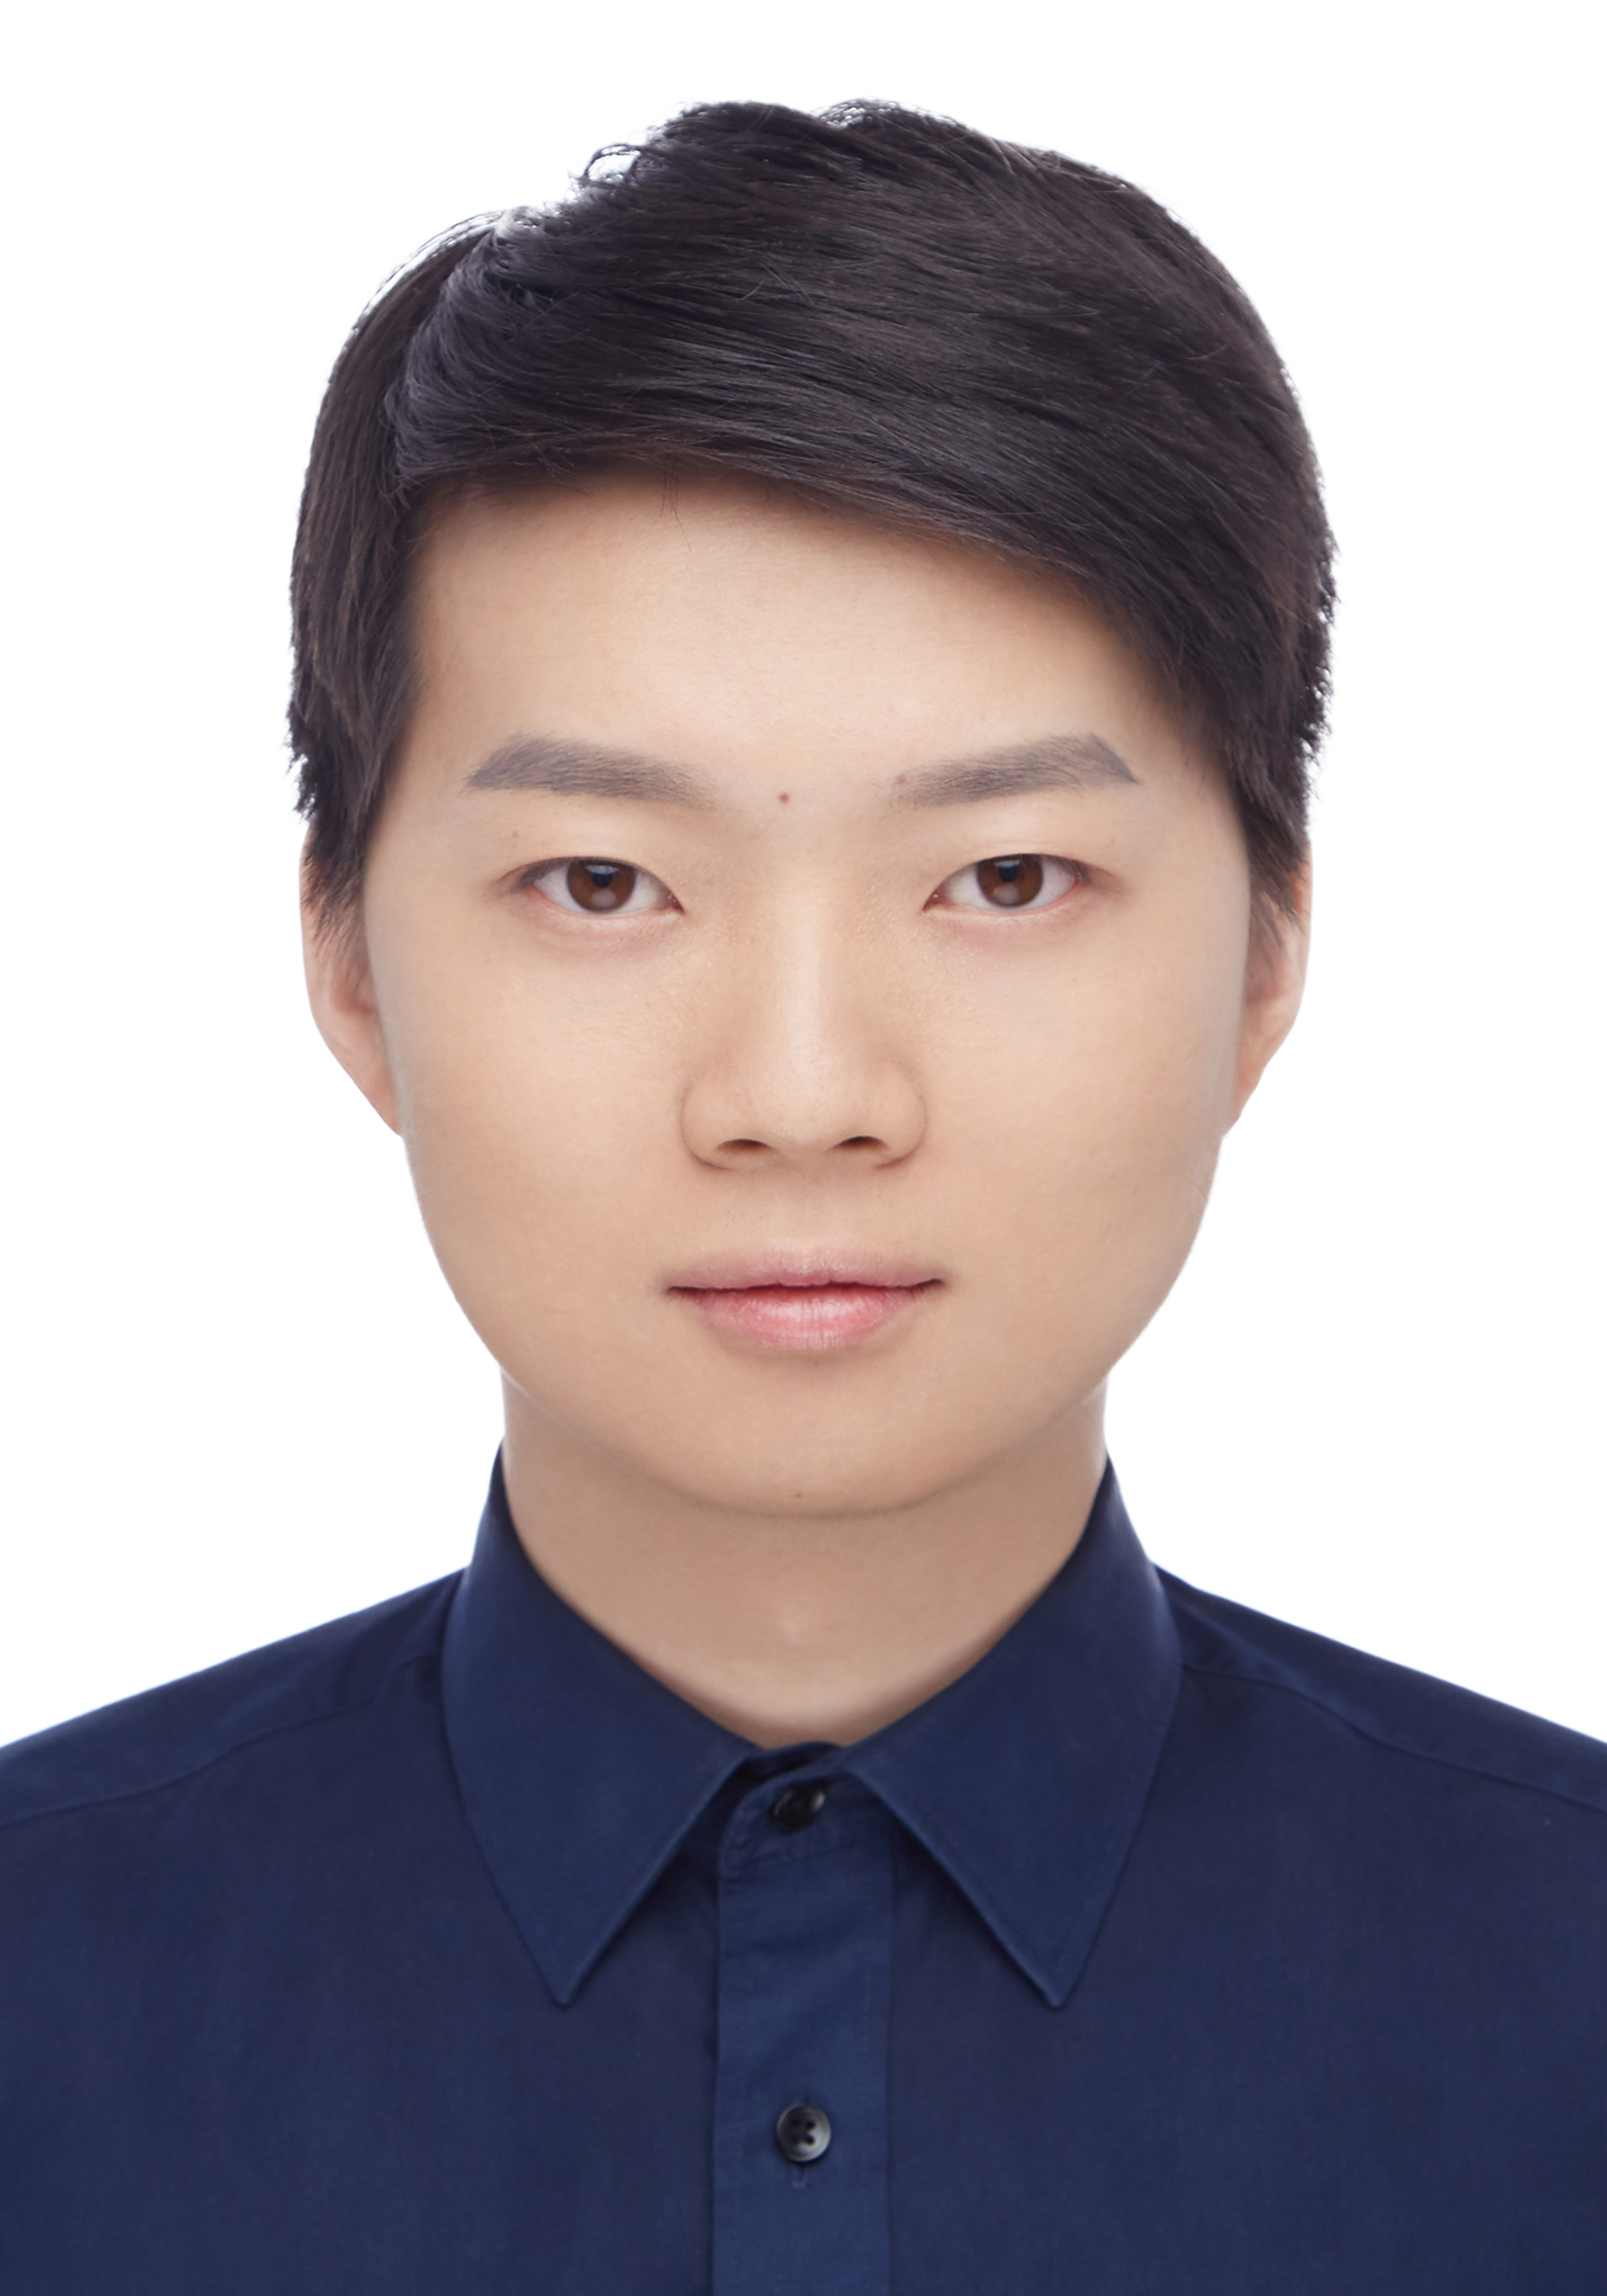
\includegraphics[height=30mm]{证件照1.jpg}
\end{minipage}

\medskip\noindent
\section{\faGraduationCap\  教育背景}
\datedsubsection{\textbf{北京航空航天大学}, 北京}{2017年9月 -- 至今}
\textit{在读硕士研究生}\quad{电子信息工程学院 \quad 专业:信息与通信工程}
\item{\quad \quad \quad \quad \quad \quad \quad \quad 通信专业学术型硕士研究生考试总成绩前十录取 , 预计2020年1月毕业}\newline
\textit{主修课程}\quad{\quad \quad \quad 时间序列与谱分析,检测、估计与调制理论等}


\datedsubsection{\textbf{北京航空航天大学}, 北京}{2013年9月 -- 2017年6月}
\textit{学士学位(本科)}\quad  {电子信息工程学院}\quad {专业:电子信息}\newline
\textit{主修课程}\quad{\quad \quad \quad c语言,计算机软件基础,通信原理,离散时间信号处理等}
\section{\faHeartO\ 获奖情况}
\datedline{\textit{北京航空航天大学研究生学业奖学金}}{2017 年 9 月}

\section{\faGraduationCap\ 学术成果}
\datedline{\textit{全国信号和智能信息处理与应用学术会议:《基于微动特征的道路场景运动目标分类》}}{2019 年 7 月}
\section{\faUsers\ 实习/项目经历}

\datedsubsection{\textbf{实习:华为北研所-海思Kirin芯片及技术开发部}}{2019年6月 -- 至今}
\role{C语言,ISP软件组}{助理工程师}
\begin{itemize}[topsep = 0 pt, partopsep = 0pt]
  \item 学习并掌握ISP软件整个系统的调度流程和运行机制
  \item 参与某Kirin芯片项目中ISP子系统下CE及LSC模块的软件驱动开发
  \item 参与CE以及LSC模块的功能修改与ut验证
\end{itemize}


\datedsubsection{\textbf{与中电29所合作,航线规划及推演软件开发项目}}{2018年3月 -- 2018年6月}
\role{C++,BCG控件}{实验室项目}
\begin{itemize}[topsep = 0 pt, partopsep = 0pt]
  \item MFC原有框架与BCG扩展控件相结合,搭建完整的用户界面
  \item 态势图上的实时航点标绘,航线编辑,航线数据处理
  \item 航线编辑完成后的模拟推演,给出分析统计结果
\end{itemize}

\datedsubsection{\textbf{空间背景软件开发项目}}{2017年10月 -- 2018年1月}
\role{C++,MFC}{实验室项目}
%\begin{onehalfspacing}
\begin{itemize}[topsep = 0 pt, partopsep = 0pt]
  \item 利用C++ MFC框架,实现软件所需要的界面显示
  \item 根据算法,展示在不同观测条件下视场内的恒星成像情况
  \item 后期进行算法优化,去除了重复的冗余计算
\end{itemize}
%\end{onehalfspacing}
\datedsubsection{\textbf{毫米波雷达运动目标检测与分类研究}}{2018年7月 -- 至今}
\role{数字信号处理,类决策树}{研究生实验室课题}
%\begin{onehalfspacing}
\begin{itemize}[topsep = 0 pt, partopsep = 0pt]
  \item 道路场景下对回波进行信号分析,给出目标信息
  \item 提取目标特征,结合宏观以及微动信息进行目标分类
  \item 实测数据处理与论文同步完成
\end{itemize}
%\end{onehalfspacing}




\section{\faCogs\ 技能}
% increase linespacing [parsep=0.5ex]
\begin{itemize}[parsep=0.5ex]
  \item 编程语言:常用 C/C++、Python、MATLAB  
  \item 系统平台及工具: Windows、Linux、Git
  \item 技能:数字信号处理、软件开发、操作系统、雷达信号分析
  \item 算法:掌握常用的算法与数据结构,了解常用的机器学习算法
  \item 英语:良好的英语听说能力,可以熟练与人交流合作 (CET-6)
  \item  办公:熟练掌握各种办公软件的使用
  \item  性格爱好:热情活波、团队意识强;喜欢体育运动(足球等)
\end{itemize}



\end{document}
